\documentclass{beamer}

\usepackage{beamerthemesplit}
\usepackage{latexsym}
\usepackage{eurosym}
\usepackage[activeacute,spanish]{babel}
\usepackage{ae,aecompl}
\usepackage{graphicx}
\usepackage{amsfonts}

\usetheme{Darmstadt}

\title{Descripcion de Proyecto -  Lenguaje de Programacion}
\author{G. Chavez - K. Campuzano - J. Camacho - K. Altamirano}
\date{\today}

\begin{document}

\frame{\titlepage}

\section[Indice]{}
\begin{frame}[allowframebreaks]
\tableofcontents
\end{frame}
%\frame{\tableofcontents}

\section{Descripcion}

  \begin{frame}
   Se trata de implementar una aplicacion movil complementaria al sistema de compra de snacks de un cine, el cliente al ingresar a la aplicacion se encontrara con todos los snacks que esten disponible para la venta al consumidor que en nuestro caso es el cliente.

El cliente para ser atendido debera ingresar a la aplicacion y escoger lo que quisiera pedir, despues de esto se le solicitaria datos necesarios como son el numero de asiento y el numero de sala para que el pedido sea llevado a su asiento.

La cancelacion de la orden se hara mediante una cuenta que el cliente debe de tener en el cine, de esta se debitara lo correspondiente al pedido y se empezara hacer la orden.

Los datos que irian en la factura son datos que previamente ha ingresado en su cuenta como son su numero de cedula, nombre,apellido,direccion,telefono y otros.. .

  \end{frame}





\section{Prototipo}
\begin{frame}[allowframebreaks]
\frametitle{Prototipo}
\begin{figure}[h]
\centering

\includegraphics[height=1.0\textheight]{main.png}
\end{figure}
\end{frame}

\begin{frame}[allowframbreaks]
\frametitle{Prototipo}
\begin{figure}[h]
\centering
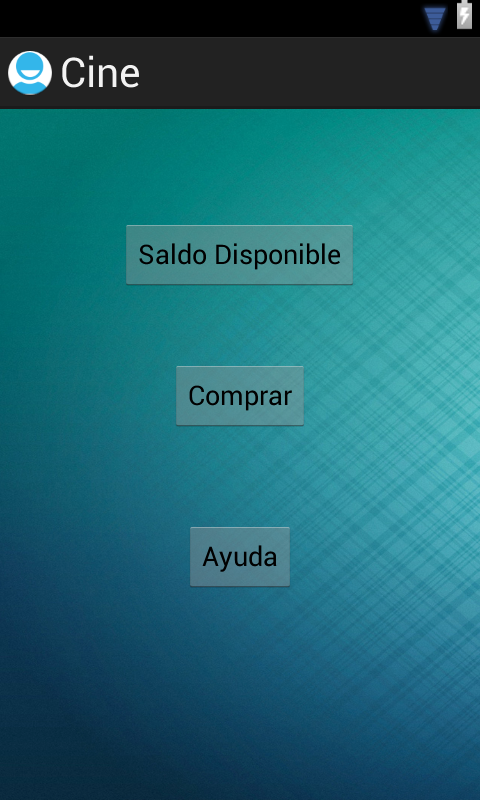
\includegraphics[height=1.0\textheight]{menu.png}
\end{figure}
\end{frame}

\begin{frame}[allowframbreaks]
\frametitle{Prototipo}
\begin{figure}[h]
\centering

\includegraphics[height=1.0\textheight]{saldo.png}
\end{figure}
\end{frame}

\begin{frame}[allowframbreaks]
\frametitle{Prototipo}
\begin{figure}[h]
\centering
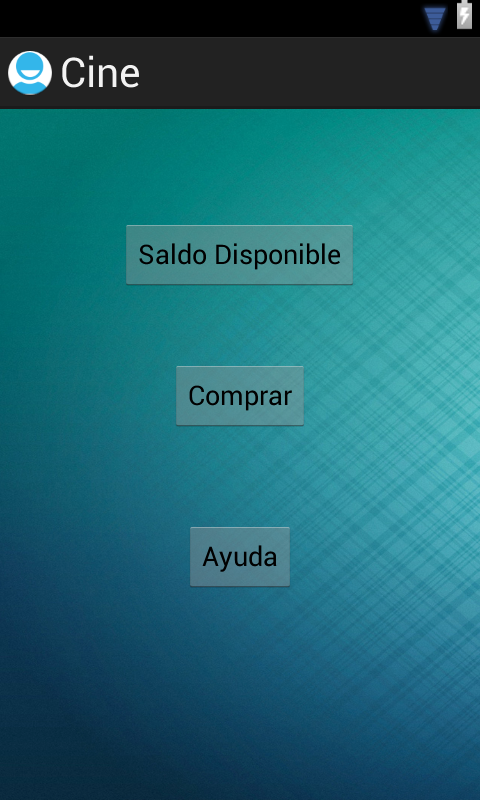
\includegraphics[height=1.0\textheight]{menu.png}
\end{figure}
\end{frame}

\begin{frame}[allowframbreaks]
\frametitle{Prototipo}
\begin{figure}[h]
\centering
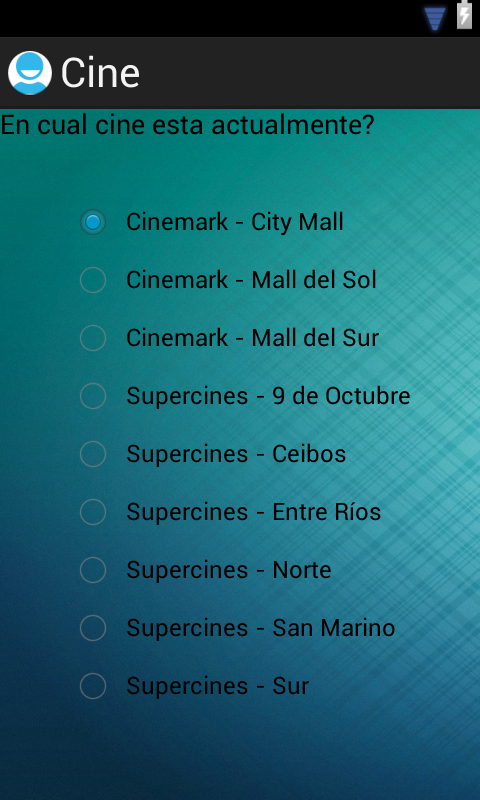
\includegraphics[height=1.0\textheight]{comprar_cine.png}
\end{figure}
\end{frame}

\begin{frame}[allowframbreaks]
\frametitle{Prototipo}
\begin{figure}[h]
\centering
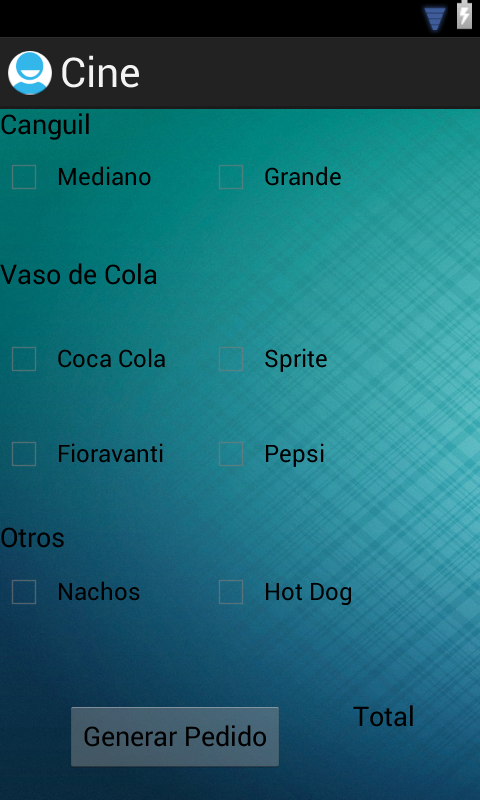
\includegraphics[height=1.0\textheight]{orden_compra.png}
\end{figure}
\end{frame}

\end{document}